\chapter{Modelo Físico} 

\begin{description}

	\item[Tipo de sistema:] Web.
	\item[Software requerido:]Apache, Maria-DB,google-chrome,firefox,edge.
	\item[OS:] Arch Linux x86\_64.
	\item[Kernel Release:] 4.14.47-1-MANJARO.
	\item[RAM:] 2006 MB / 3835 MB
	\item[Processor Type:] Intel(R) Celeron(R) CPU B830 @ 1.80GHz.
	\item[servicios:] servicios del servidor de base de datos 10.1.33-MariaDB MariaDB Server.\\También se Ocupan servicios del serve API Apache 2.0 Handler
Con la Version de Apache:	Apache/2.4.33 (Unix) PHP/7.2.6.
	\item[Mysql Support:] mysqlnd 5.0.12-dev - 20150407.
	\item[Hosting:]Se Compra un servidor dedicado con el proveedor ``Go Daddy".
	Se compra un servidor dedicado, para que se pueda dar soporte a  todos los empleados en todas las sucursales, tal vez al principio se tendrá espacio y servidor de sobra, pero de esta forma aumenta la productividad y se quitan los riesgos de tráfico en el servidor.
	\item[servidor Hosting:]4 núcleos de CPU @ 3.1 GHz
Memoria de 4 GB
1 TB de almacenamiento (RAID-1)\^
Ancho de banda sin medición(El proveedor no limita el ancho de banda) 
3 IP dedicadas
Certificado SSL gratis durante 1 año.
	\item[Dominio:] Se Compra el dominio ``www.Farmacias.francs.com"\\  con el mismo proveedor a un precio muy razonable con contrato de un año al igual que el servicio de hosting.
	\item[Seguridad web:]El mismo proveedor de hosting ofrece seguridad SSL
	con las siguientes Características:Asegura un sitio web
Sólido cifrado SHA2 y encriptación de 2048 bits\\
Disponible en Certificados SSL DV, OV y EV.\\
El SSL EV hace que la barra del navegador se ponga verde 
Incrementa el posicionamiento de tu sitio en Google.\\
Marca confiable McAfee SECURE.\\
\end{description}
\begin{figure}[htbp!]
	\begin{center}
		\fbox{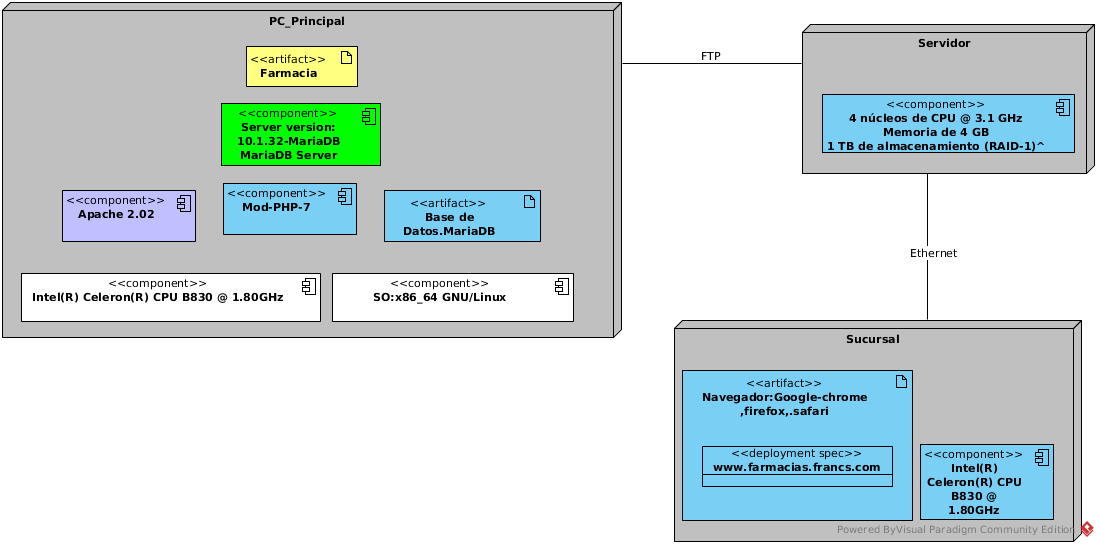
\includegraphics[width=18cm, height=20cm]{images/arquitectura}}
		\caption{Arquitectura del sistema.}
		\label{fig:arquitectura}
	\end{center}
\end{figure}

En la figura~\ref{fig:arquitectura} se describe la estructura del sistema, en ella se detallan los servicios de base de datos que se necesitan, las conexiones al servidor apache, así como las especificaciones que necesita el CPU de la sucursal en la que se monta el sistema de la farmacia.
